\documentclass{standalone}
\usepackage{tikz}
\usetikzlibrary{patterns, positioning}


\begin{document}
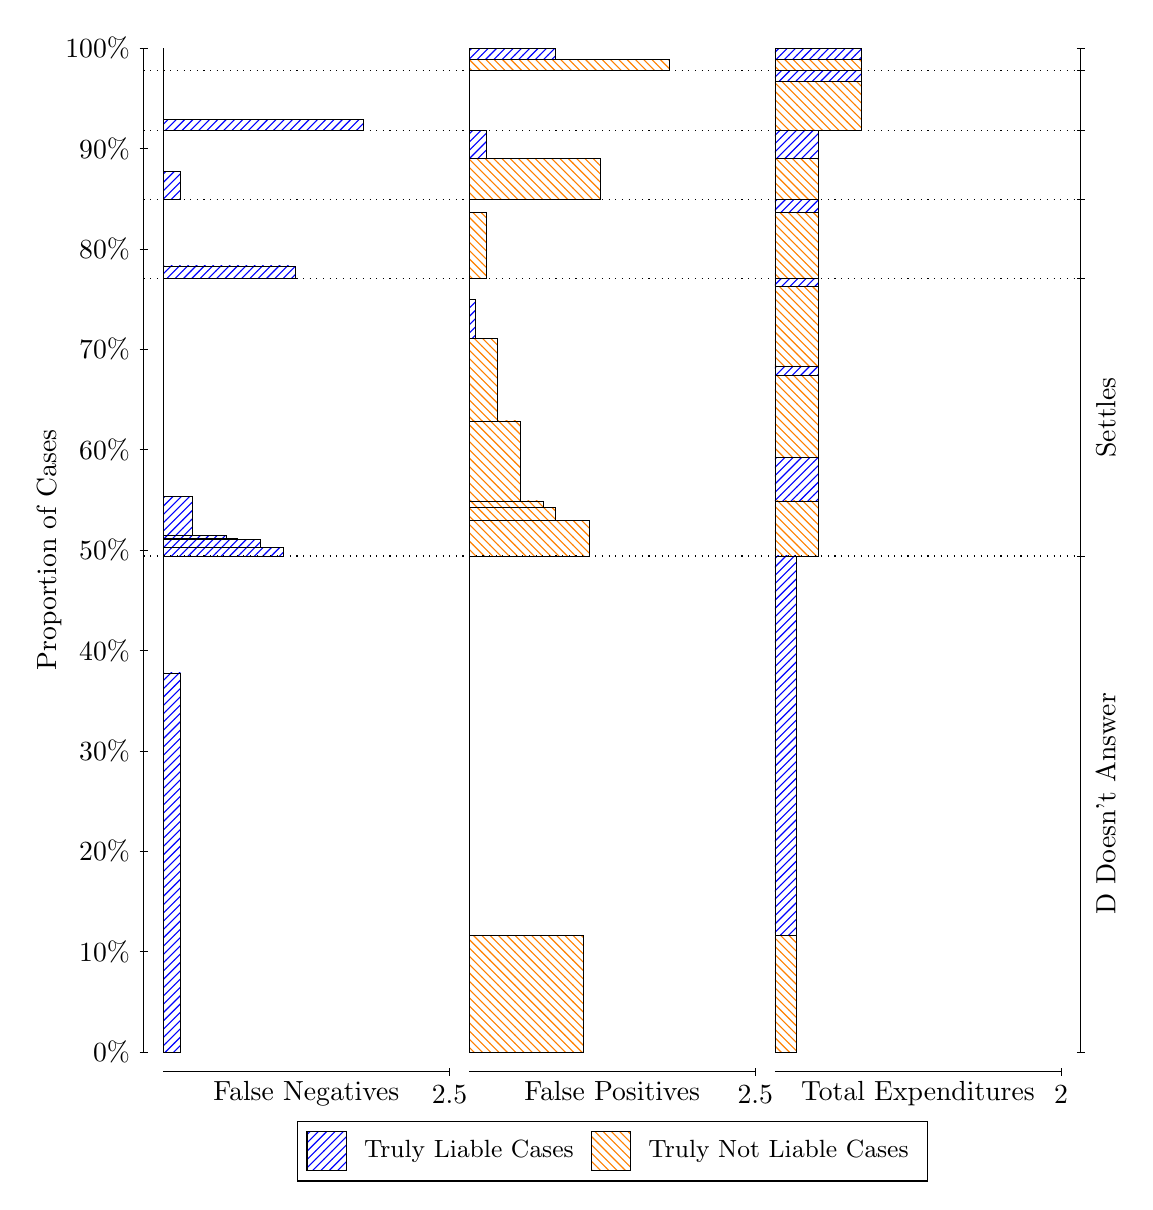
\begin{tikzpicture}
\draw[black, very thin] (1.5,1.75) -- (1.5,14.5);
\node[rotate=90, text=black, anchor=center] at (0.3, 8.125) {Proportion of Cases};
\draw[black, very thin] (1.45,1.75) -- (1.55,1.75);
\node[text=black, anchor=east] at (1.45, 1.75) {0\%};
\draw[black, very thin] (1.45,3.025) -- (1.55,3.025);
\node[text=black, anchor=east] at (1.45, 3.025) {10\%};
\draw[black, very thin] (1.45,4.3) -- (1.55,4.3);
\node[text=black, anchor=east] at (1.45, 4.3) {20\%};
\draw[black, very thin] (1.45,5.575) -- (1.55,5.575);
\node[text=black, anchor=east] at (1.45, 5.575) {30\%};
\draw[black, very thin] (1.45,6.85) -- (1.55,6.85);
\node[text=black, anchor=east] at (1.45, 6.85) {40\%};
\draw[black, very thin] (1.45,8.125) -- (1.55,8.125);
\node[text=black, anchor=east] at (1.45, 8.125) {50\%};
\draw[black, very thin] (1.45,9.4) -- (1.55,9.4);
\node[text=black, anchor=east] at (1.45, 9.4) {60\%};
\draw[black, very thin] (1.45,10.675) -- (1.55,10.675);
\node[text=black, anchor=east] at (1.45, 10.675) {70\%};
\draw[black, very thin] (1.45,11.95) -- (1.55,11.95);
\node[text=black, anchor=east] at (1.45, 11.95) {80\%};
\draw[black, very thin] (1.45,13.225) -- (1.55,13.225);
\node[text=black, anchor=east] at (1.45, 13.225) {90\%};
\draw[black, very thin] (1.45,14.5) -- (1.55,14.5);
\node[text=black, anchor=east] at (1.45, 14.5) {100\%};

\draw[black, very thin] (13.4,1.75) -- (13.4,14.5);
\draw[black, very thin] (13.35,1.75) -- (13.45,1.75);
\node[anchor=west] at (13.35, 1.75) {};
\draw[black, very thin] (13.35,8.0489) -- (13.45,8.0489);
\node[anchor=west] at (13.35, 8.0489) {};
\draw[black, very thin] (13.35,11.57) -- (13.45,11.57);
\node[anchor=west] at (13.35, 11.57) {};
\draw[black, very thin] (13.35,12.577) -- (13.45,12.577);
\node[anchor=west] at (13.35, 12.577) {};
\draw[black, very thin] (13.35,13.451) -- (13.45,13.451);
\node[anchor=west] at (13.35, 13.451) {};
\draw[black, very thin] (13.35,14.22) -- (13.45,14.22);
\node[anchor=west] at (13.35, 14.22) {};
\draw[black, very thin] (13.35,14.5) -- (13.45,14.5);
\node[anchor=west] at (13.35, 14.5) {};

\draw[black, very thin, pattern color=blue, pattern=north east lines] (1.75,1.75) rectangle (1.968,6.5651);
\draw[black, very thin, pattern color=orange, pattern=north west lines] (1.75,6.5651) rectangle (1.75,8.0489);
\draw[black, very thin, pattern color=blue, pattern=north east lines] (1.75,8.0489) rectangle (3.276,8.1555);
\draw[black, very thin, pattern color=blue, pattern=north east lines] (1.75,8.1555) rectangle (2.9853,8.2552);
\draw[black, very thin, pattern color=blue, pattern=north east lines] (1.75,8.2552) rectangle (2.6947,8.2749);
\draw[black, very thin, pattern color=blue, pattern=north east lines] (1.75,8.2749) rectangle (2.5493,8.3075);
\draw[black, very thin, pattern color=blue, pattern=north east lines] (1.75,8.3075) rectangle (2.1133,8.8082);
\draw[black, very thin, pattern color=orange, pattern=north west lines] (1.75,8.8082) rectangle (1.75,11.57);
\draw[black, very thin, pattern color=blue, pattern=north east lines] (1.75,11.57) rectangle (3.4213,11.734);
\draw[black, very thin, pattern color=orange, pattern=north west lines] (1.75,11.734) rectangle (1.75,12.577);
\draw[black, very thin, pattern color=blue, pattern=north east lines] (1.75,12.577) rectangle (1.968,12.932);
\draw[black, very thin, pattern color=orange, pattern=north west lines] (1.75,12.932) rectangle (1.75,13.451);
\draw[black, very thin, pattern color=blue, pattern=north east lines] (1.75,13.451) rectangle (4.2933,13.591);
\draw[black, very thin, pattern color=orange, pattern=north west lines] (1.75,13.591) rectangle (1.75,14.22);
\draw[black, very thin, pattern color=orange, pattern=north west lines] (1.75,14.22) rectangle (1.75,14.358);
\draw[black, very thin, pattern color=blue, pattern=north east lines] (1.75,14.358) rectangle (1.75,14.5);
\draw[black, very thin, pattern color=orange, pattern=north west lines] (5.6333,1.75) rectangle (7.0867,3.2338);
\draw[black, very thin, pattern color=blue, pattern=north east lines] (5.6333,3.2338) rectangle (5.6333,8.0489);
\draw[black, very thin, pattern color=orange, pattern=north west lines] (5.6333,8.0489) rectangle (7.1593,8.5013);
\draw[black, very thin, pattern color=orange, pattern=north west lines] (5.6333,8.5013) rectangle (6.7233,8.6701);
\draw[black, very thin, pattern color=orange, pattern=north west lines] (5.6333,8.6701) rectangle (6.578,8.7482);
\draw[black, very thin, pattern color=orange, pattern=north west lines] (5.6333,8.7482) rectangle (6.2873,9.7651);
\draw[black, very thin, pattern color=orange, pattern=north west lines] (5.6333,9.7651) rectangle (5.9967,10.811);
\draw[black, very thin, pattern color=blue, pattern=north east lines] (5.6333,10.811) rectangle (5.706,11.311);
\draw[black, very thin, pattern color=blue, pattern=north east lines] (5.6333,11.311) rectangle (5.6333,11.57);
\draw[black, very thin, pattern color=orange, pattern=north west lines] (5.6333,11.57) rectangle (5.8513,12.413);
\draw[black, very thin, pattern color=blue, pattern=north east lines] (5.6333,12.413) rectangle (5.6333,12.577);
\draw[black, very thin, pattern color=orange, pattern=north west lines] (5.6333,12.577) rectangle (7.3047,13.096);
\draw[black, very thin, pattern color=blue, pattern=north east lines] (5.6333,13.096) rectangle (5.8513,13.451);
\draw[black, very thin, pattern color=orange, pattern=north west lines] (5.6333,13.451) rectangle (5.6333,14.08);
\draw[black, very thin, pattern color=blue, pattern=north east lines] (5.6333,14.08) rectangle (5.6333,14.22);
\draw[black, very thin, pattern color=orange, pattern=north west lines] (5.6333,14.22) rectangle (8.1767,14.358);
\draw[black, very thin, pattern color=blue, pattern=north east lines] (5.6333,14.358) rectangle (6.7233,14.5);
\draw[black, very thin, pattern color=orange, pattern=north west lines] (9.5167,1.75) rectangle (9.7892,3.2338);
\draw[black, very thin, pattern color=blue, pattern=north east lines] (9.5167,3.2338) rectangle (9.7892,8.0489);
\draw[black, very thin, pattern color=orange, pattern=north west lines] (9.5167,8.0489) rectangle (10.062,8.7482);
\draw[black, very thin, pattern color=blue, pattern=north east lines] (9.5167,8.7482) rectangle (10.062,9.3011);
\draw[black, very thin, pattern color=orange, pattern=north west lines] (9.5167,9.3011) rectangle (10.062,10.347);
\draw[black, very thin, pattern color=blue, pattern=north east lines] (9.5167,10.347) rectangle (10.062,10.453);
\draw[black, very thin, pattern color=orange, pattern=north west lines] (9.5167,10.453) rectangle (10.062,11.47);
\draw[black, very thin, pattern color=blue, pattern=north east lines] (9.5167,11.47) rectangle (10.062,11.57);
\draw[black, very thin, pattern color=orange, pattern=north west lines] (9.5167,11.57) rectangle (10.062,12.413);
\draw[black, very thin, pattern color=blue, pattern=north east lines] (9.5167,12.413) rectangle (10.062,12.577);
\draw[black, very thin, pattern color=orange, pattern=north west lines] (9.5167,12.577) rectangle (10.062,13.096);
\draw[black, very thin, pattern color=blue, pattern=north east lines] (9.5167,13.096) rectangle (10.062,13.451);
\draw[black, very thin, pattern color=orange, pattern=north west lines] (9.5167,13.451) rectangle (10.607,14.08);
\draw[black, very thin, pattern color=blue, pattern=north east lines] (9.5167,14.08) rectangle (10.607,14.22);
\draw[black, very thin, pattern color=orange, pattern=north west lines] (9.5167,14.22) rectangle (10.607,14.358);
\draw[black, very thin, pattern color=blue, pattern=north east lines] (9.5167,14.358) rectangle (10.607,14.5);
\draw[black, dotted] (1.5,8.0489) -- (13.4,8.0489);
\draw[black, dotted] (1.5,11.57) -- (13.4,11.57);
\draw[black, dotted] (1.5,12.577) -- (13.4,12.577);
\draw[black, dotted] (1.5,13.451) -- (13.4,13.451);
\draw[black, dotted] (1.5,14.22) -- (13.4,14.22);
\draw[black, very thin] (1.75,1.5) -- (5.3833,1.5);
\node[text=black, anchor=north] at (3.5667, 1.5) {False Negatives};
\draw[black, very thin] (5.3833,1.45) -- (5.3833,1.55);
\node[text=black, anchor=north] at (5.3833, 1.45) {2.5};

\draw[black, very thin] (5.6333,1.5) -- (9.2667,1.5);
\node[text=black, anchor=north] at (7.45, 1.5) {False Positives};
\draw[black, very thin] (9.2667,1.45) -- (9.2667,1.55);
\node[text=black, anchor=north] at (9.2667, 1.45) {2.5};

\draw[black, very thin] (9.5167,1.5) -- (13.15,1.5);
\node[text=black, anchor=north] at (11.333, 1.5) {Total Expenditures};
\draw[black, very thin] (13.15,1.45) -- (13.15,1.55);
\node[text=black, anchor=north] at (13.15, 1.45) {2};

\node[text=black, centered, rotate=90] at (13.72, 4.8994) {D Doesn't Answer};
\node[text=black, centered, rotate=90] at (13.72, 9.8094) {Settles};





\draw (7.449999999999999,1.5) node[draw=none] (baseCoordinate) {};
\begin{scope}[align=center]
        \matrix[scale=0.5, draw=black, below=0.5cm of baseCoordinate, nodes={draw}, column sep=0.1cm]{
            \node[rectangle, draw, minimum width=0.5cm, minimum height=0.5cm, pattern color=blue, pattern=north east lines] {}; &
            \node[draw=none, font=\small, text=black] (B) {Truly Liable Cases}; &
            \node[rectangle, draw, minimum width=0.5cm, minimum height=0.5cm, pattern color=orange, pattern=north west lines] {}; &
            \node[draw=none, font=\small, text=black] (B) {Truly Not Liable Cases}; \\
            };
\end{scope}

\end{tikzpicture}
\end{document}